\documentclass[conference]{IEEEtran}
\usepackage{graphicx} % Required for inserting images
\usepackage{epstopdf}
\usepackage{float}
\usepackage{verbatim}
\usepackage{array}
\usepackage{authblk}
% \usepackage{IEEEtrantools}
\usepackage[
    backend=biber,
    style=ieee,
  ]{biblatex}
\addbibresource{additional.bib}  % Additional papers (those not found in SLR)
\usepackage{svg}

\usepackage{xcolor}
\usepackage{longtable}

\begin{document}

\title{Performance Analysis of Cache Size and Set-Associativity Using gem5}

\author[1]{Clayton Asada}
\author[2]{Joseph Chorbajian}
\author[3]{Ilmaan Zia}

\affil[1,2,3]{Computer Engineering and Computer Science, California State University Long Beach}

\date{February 2023}



\maketitle



\begin{abstract}
% TODO: Maybe include most prominent results/analyses in abstract?

\emph{Keywords - } Cache, Size, Associativity, Replacement Policy, gem5, Simulation, Configuration, Miss rate
\end{abstract}

% THIS IS LEFT HERE AS AN EXAMPLE/TEMPLATE FOR INCLUDING PICTURES
% \begin{figure}[H]
%     \centering
%     \includegraphics[width=0.45\textwidth]{images/EmpC1-Training}
%     \caption{Amount of training provided}
%     \label{fig:EmpC1-Training}
% \end{figure}

\section{Introduction}

Cache performance is critical to the performance and efficiency of modern computer systems. As processors have become increasingly fast, the memory and storage hierarchy have struggled to keep up, leading to a performance gap between processors and memory systems. Caches are small, fast memories that sit between the processor and main memory to help bridge this performance gap and supply the processor with data and instructions quickly\cite{hennessy_computer_2012}.

The design of caches involves navigating multiple trade-offs between cache size, associativity, block size, and replacement policies in order to achieve optimal performance for a given workload. Larger cache sizes can store more data, reducing the number of slow accesses to main memory, but have other trade-offs such as having higher access latencies and consuming more power. Associativity refers to the number of locations in the cache that can store a given memory block. Higher associativity reduces conflict misses that occur when two memory blocks map to the same cache location, exchanging for additional hardware cost. Block size determines how much data is brought into the cache at once on a cache miss. Larger block sizes can improve spatial locality and reduce miss rates, but they also bring in more unused data, wasting cache space. Replacement policies determine which cache line is evicted when the cache is full and a new memory block needs to be brought in. More effective replacement policies can improve cache miss rate by reducing the number of useful cache lines evicted\cite{hennessy_computer_2012}.

Simulation tools, like gem5\cite{10.1145/2024716.2024718} and SimpleScalar\cite{10.1145/268806.268810}, are useful for exploring the cache design space and evaluating trade-offs. These tools run simulated workloads and collect various cache metrics across different configurations. This allows designers to find the optimal balance of size, associativity, block size, and replacement policy for a target workload without having to build physical hardware prototypes.

In this paper, we show optimizations of cache miss rates through navigation of these trade-offs. We compare the miss rates on a total of 72 configurations per benchmark by varying cache size, associativity, block size, and replacement policies. Other cache parameters have remained constant. We use three benchmarks from the MiBench benchmark suite, designed for embedded processors. As such, the cache size, block size, and set associativity all match appropriate configurations for embedded processors.

\section{Related Work}

As cache performance is crucial for modern computer systems, computer architecture researchers community has recognized its significance. As a result, cache design has been extensively studied and optimized to improve system performance, with researchers exploring various cache configurations through simulation over decades.

For instance, researchers have explored trade-offs between cache replacement policies. In 2004, Al-Zoubi et. al.\cite{10.1145/986537.986601} evaluated cache replacement policies on the CPU2000 benchmark suite using SimpleScalar and found that LRU and LRU-based policies, specifically pseudo-LRU replacement policies, performed best. More recent studies by Panda et. al.\cite{7806218} shows that modern LRU-based replacement policies outperforming pseudo-LRU using the CPU2006 benchmarks.

Cache size has also been extensively studied. Ma et. al.\cite{5260945} used SimpleScalar to evaluate miss rates across multiple benchmarks in SPEC2000 and found that a larger L1 cache size significantly improves performance when the cache size is small, but gradually decreases as the cache gets bigger. Ullah et. al.\cite{8975563} built on this work by proposing a 2:1 cache rule of thumb, which states that the miss rates of a cache with $n$ cache size and $x$ associativity are equivalent to the miss rates on a configuration with $n/2$ cache size and $2x$ associativity.

While most research on cache configurations and miss rates have been done in SimpleScalar, some research has used gem5. Reas et. al.\cite{10.1109/UKSIM.2010.35} have simulated L2 cache miss rates on m5 (the precursor to gem5) and compared them to miss rates on hardware implementations of their design on the SPLASH-2 benchmark suite.

\section{Motivation}

As stated before, cache performance is a critical factor for any computer system as it plays a significant role in improving system performance and energy efficiency, particularly in memory-intensive workloads. This becomes a greater issue for embedded processors, where speed and energy efficiency have high priority. Therefore, understanding the trade-offs between cache size, associativity, block size, and replacement policies is crucial in the optimization process for processor design.

Furthermore, many simulations of miss rates for various processor configurations use SimpleScalar\cite{10.1145/268806.268810} as their simulator of choice. Original versions of SimpleScalar used its own instruction set architecture derived from MIPS-IV ISA\cite{10.1145/268806.268810} and may not necessarily model real-world processors accurately. While there has been significant research on porting SimpleScalar to different architectures, such as PowerPC, x86, and ARM\cite{10.1145/986537.986601} (with ARM being verified as cycle-accurate\cite{CHUNG2006137}), most research papers on simulating miss rates do not specify the version of SimpleScalar used, the computing environment used, or the instruction set architecture it was ran on.

Therefore, we have developed key questions that our paper hopes to answer:

\begin{enumerate}
  \item What is the best configuration for embedded processors on the selected benchmarks?
  \item Does the 2:1 cache rule of thumb hold for the selected benchmarks?
  \item How does gem5 and SimpleScalar differ on simulated cache miss rates?
\end{enumerate}

Our research aims to contribute to the understanding of cache performance and design by using the gem5 simulator to model various single-core CPU cache configurations. To evaluate the effectiveness of gem5 in modeling cache performance compared to SimpleScalar, we base our configurations on configurations used in Ullah et. al.. In addition, we also aim to explore the impact of replacement policies on cache performance. By comparing the results of our study with those of Ullah et. al., we hope to provide a comprehensive picture of cache performance across different simulators and identify any differences in their respective results.

Our research has the potential to inform cache design and optimization, as well as guide future research in this area. By understanding the impact of cache size, associativity, block size, and replacement policies on performance, we can design more effective caches that improve system performance and energy efficiency. Furthermore, by evaluating the effectiveness of simulation tools such as gem5 and SimpleScalar, we can improve the accuracy and efficiency of cache performance modeling.

\section{Research methodology}
In this research, we use the gem5 simulator to model various single-core CPU cache configurations and evaluate their performance under different workloads. We describe the experimental methodology below.

Hardware and Software Configuration:
We use a Linux-based system for our experiments as that is a base requirement for the gem5 simulator. Additionally the research team purposefully used different types of hardware and operating systems to run the simulations to determine if there were any inconsistencies in the gem5 simulator. Two desktop computers, one operating on Ubuntu 22.04 and the other Debian distro, and a third laptop using WSL were used to run the gem5 simulations. We use gem5 version 20.0.0 for our simulations.

Workloads:
We use a variety of benchmark workloads to evaluate the performance of different cache configurations. The specific benchmarks used in this research are Dijkstra, Sha, and Rijndael from the SPEC95 benchmark quite. The previous paper used two additional workloads, Go and Compress.

Cache Configurations:
We evaluate several cache configurations with different sizes, different block sized, associativity, and replacement policies. As seen in the cache sizes configurations used were 16kB, 32kB, and 64kB. Cache block sizes were configuratble to 32 bytes and 64 bytes. The final configurations that were used for the original research was set associativities of 1, 2, 4, and 8. The additional configuration used in this study beyond what the original tested are following replacement policies, least recently used, random replacement, and first in first out replacement policy.

We use the findings of the previous research paper as a baseline for comparison of each unique combination of configurations.

Table \ref{table:configurations} shows the various configurations tested. The three benchmarks come from the MiBench benchmark suite, designed for embedded processors\cite{990739}. Least Recently Used (LRU), Random, and First-In First-Out (FIFO) are common replacement policies. While there are other replacement policies that may be better, 

\begin{table}[H]
  \centering
  \begin{tabular}{| m{1.6cm} | m{.75cm} | m{.75cm} | m{.8cm} | m{2.6cm} |}
      \hline
      \textbf{Benchmarks} & \textbf{Cache Size} & \textbf{Block Size}& \textbf{Set Assoc.}& \textbf{Replacement Policy} \\ \hline
      Dijkstra    &   16kB  &   32    &  1   &    Least Recently Used     \\ \hline
      Sha         &   32kB  &   64    &  2   &    Random                  \\ \hline
      Rijndael    &   64kB  &         &  4   &    First-In First-Out      \\ \hline
                  &         &         &  8   &                            \\ \hline
  \end{tabular}
  \caption{The different configurations tested.}
  \label{table:configurations}
\end{table}

Simulation Setup:
We use gem5's full-system mode to simulate our experiments. In this mode, the entire system, including the CPU, cache, and memory hierarchy, is simulated. We run each workload multiple times to ensure the stability of the results and use a warm-up period to ensure that the cache is populated before we start collecting performance data.

Performance Metrics:
We collect several performance metrics, including execution time, instruction throughput, and cache hit rate. We also collect cache miss rate, cache eviction rate, and average memory access latency to provide a more detailed analysis of cache behavior.

Statistical Analysis:
We use statistical analysis to compare the performance of different cache configurations. We use the t-test to determine if there are statistically significant differences between the performance of different configurations. We also use analysis of variance (ANOVA) to determine the impact of different cache parameters on performance.

In summary, our experimental methodology involves using the gem5 simulator to evaluate various single-core CPU cache configurations under different workloads. We use a range of performance metrics to compare the performance of different configurations and use statistical analysis to determine the significance of our results.

\section{Results}


\subsection{Sha Benchmark}


\subsection{Dijkstra Benchmark}


\subsection{Rijndael Benchmark}

MiBench provides an implementation of Rijndael. While modern desktop CPUs have instructions for Rijndael\cite{gueron2010intel}, they may not be implemented on embedded systems or on systems with small cache configurations. Figure \ref{fig:rijndael-cachesize} shows the miss rates on configurations with 16kB, 32kB, and 64kB of cache size and 1, 2, 4, and 8 associativity. The configuration with cache size of 16kB and an associativity of 1 shows the highest miss rate at 0.1529. It significantly improves if the cache size or the associativity changes. The miss rates with respect to cache size is monotonically decreasing. That is, a cache size of 16kB with associativity remaining the same will always perform worse than 32kB, and the same with 32kB compared to 64kB. Furthermore, miss rates with respect to associativity also monotonically decreases. The 2:1 cache rule of thumb applies for the configuration of 32kB cache size and 1 associativity compared to the 16kB cache size and 2 associativity, having miss rates 0.0424 and 0.0464, respectively. However, it quickly falls apart with configurations of 64kB cache size and 1 associativity and of 32kB cache size and 2 associativity, having miss rates 0.0353 and 0.0239. The gap continues to increase for larger configurations.

\begin{figure}[H]
    \centering
    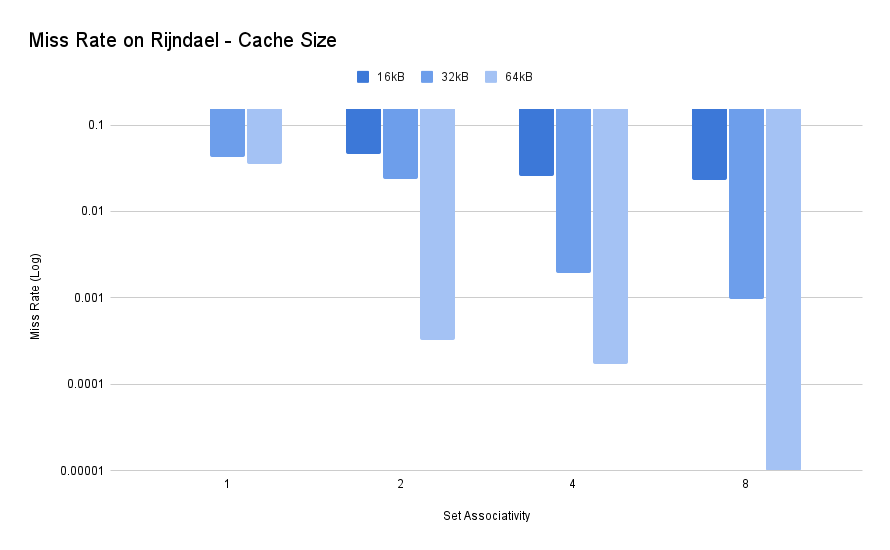
\includegraphics[width=0.45\textwidth]{images/rijndael_cachesize.png}
    \caption{The miss rate on configurations with different set associativities and cache sizes. The miss rates on the D-cache are on a logarithmic scale to represent the large disparities in the miss rates. Smaller values are better.}
    \label{fig:rijndael-cachesize}
\end{figure}

Figure \ref{fig:rijndael-blocksize} shows the miss rates on configurations with block size of either 32 or 64 and an associativity of 1, 2, 4, and 8. Unlike Figure \ref{fig:rijndael-cachesize}, the miss rates are not monotonically decreasing as the cache size or associativity increases. For an associativity of 1, the miss rates for a configuration with a block size of 32 slightly loses over a configuration of a block size of 64 (miss rates 0.0780 and 0.0758, respectively). This pattern does not hold for larger associativities. However, with the exception of an associativity of 1, the larger the associativity, the smaller the difference between the block sizes. 

\begin{figure}[H]
  \centering
  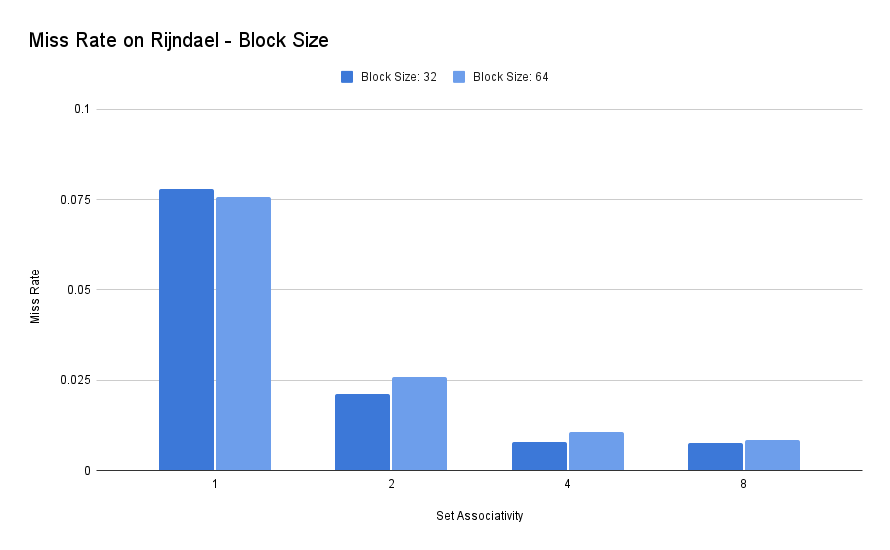
\includegraphics[width=0.45\textwidth]{images/rijndael_blocksize.png}
  \caption{The D-cache miss rate on configurations with different set associativities and block sizes. Smaller values are better.}
  \label{fig:rijndael-blocksize}
\end{figure}

This pattern is explored more in Figure \ref{fig:rijndael-missrate-percentchange}. Looking solely at the cache size, increasing block size on larger cache size often lowers miss rate. If we break down by associativity, an associativity of 1 always benefits from a larger block size, an associativity of 4 and 8 improve with larger cache sizes. The exception is a configuration with associativity of 2, as that will always benefit from a block size of 32.

\begin{figure}[H]
  \centering
  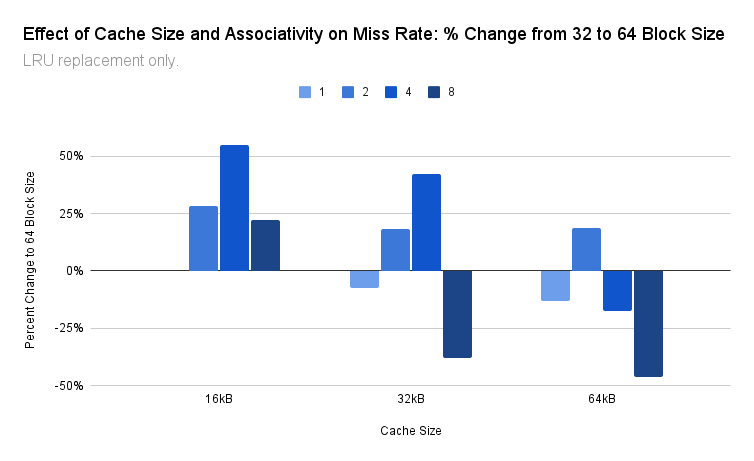
\includegraphics[width=0.45\textwidth]{images/rijndael_missrate_percentchange.png}
  \caption{The percent change of D-cache miss rate from configurations with 32 vs 64 block size. Only LRU replacement policy is shown, but the pattern remains the same with other replacement policies (although their extent differs). Smaller values are better.}
  \label{fig:rijndael-missrate-percentchange}
\end{figure}

Expanding more on the 2:1 cache rule of thumb, Figure \ref{fig:rijndael-percentdifference} shows the percent difference of "cache rule of thumb" configurations. That is, the percent difference between a configuration with $n$ cache size and $x$ associativity and a configuration with $n/2$ cache size and $2x$ associativity. A value of zero indicates that the two values are the same. If many runs exhibit a percent difference close to zero, then the cache rule of thumb would hold for Rijndael benchmarks. However, 19 out of 35 runs exhibit a percent difference of greater than 50\%, indicating a significant deviation from the supposed 2:1 cache rule of thumb.

\begin{figure}[H]
  \centering
  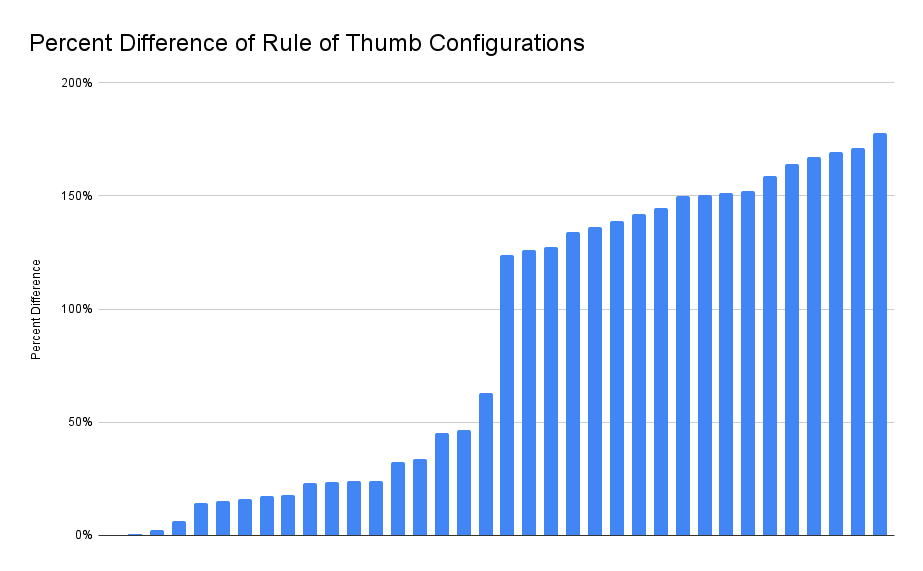
\includegraphics[width=0.45\textwidth]{images/rijndael_percentdifference.png}
  \caption{The percent difference of D-cache miss rates of cache rule of thumb configurations. Values closer to 0 are better.}
  \label{fig:rijndael-percentdifference}
\end{figure}

\section{Discussion}


\section{Future Work}
The use of gem5 to model various single-core CPU cache configurations provides a powerful tool for evaluating cache performance. Our research has shown that different cache configurations can have a significant impact on performance, and that using simulation tools such as gem5 can provide detailed insights into cache behavior.

There are several directions for future research in this area:

Multi-core CPU Cache Configurations: In this study, we focus on single-core CPU cache configurations. However, multi-core CPUs are becoming increasingly common, and cache design for multi-core CPUs is a complex and challenging area of research. Future studies could use gem5 to model various multi-core CPU cache configurations and evaluate their performance under different workloads.

Machine Learning Techniques: Recent research has explored the use of machine learning techniques to optimize cache performance. These techniques involve using machine learning algorithms to predict cache behavior and optimize cache configurations. Using gem5 to evaluate these techniques can help identify their strengths and weaknesses and guide future research in this area.

Emerging Memory Technologies: Emerging memory technologies, such as phase-change memory (PCM) and resistive random-access memory (RRAM), have the potential to revolutionize cache design. These technologies have different performance characteristics than traditional memory technologies, and designing caches that can take advantage of their unique properties is an area of active research. Future studies could use gem5 to evaluate cache designs that incorporate emerging memory technologies.

Energy-Efficient Caches: Energy efficiency is becoming an increasingly important consideration in cache design. Caches are power-hungry components of the memory hierarchy, and designing energy-efficient caches is essential to reduce power consumption and improve battery life. Future studies could use gem5 to evaluate energy-efficient cache designs, such as cache compression and cache bypassing techniques.

In conclusion, the use of gem5 to model various single-core CPU cache configurations provides a powerful tool for evaluating cache performance. Future research in this area could explore multi-core CPU cache configurations, machine learning techniques, emerging memory technologies, and energy-efficient caches. These studies could provide valuable insights into cache design and help improve the performance and energy efficiency of modern computer systems.

\section{Conclusion}
In this research, we have used the gem5 simulator to model various single-core CPU cache configurations and evaluated their performance using several benchmarks. We compared our results with those of a previous study that used the SimpleScalar simulator to evaluate cache performance. Our research aimed to contribute to the understanding of cache performance and design, as well as evaluate the effectiveness of different simulators in modeling cache behavior.

Our study found that the performance of different cache configurations varied significantly depending on the workload characteristics. We observed that the impact of replacement policies on cache performance was insignificant, with the LRU policy outperforming the FIFO and Random policies in most cases.

Our results differed significantly from those of the previous study, which focused on the impact of cache size and associativity on performance using the SimpleScalar simulator. We found that the performance of cache configurations varied depending on the simulator. Our findings suggest that the gem5 simulator may be more effective in modeling cache behavior of modern CPU's compared to SimpleScalar.

Our research has several implications for cache design and optimization. By understanding the impact of different cache configurations on performance, designers can improve system performance and energy efficiency. Our findings also have implications for the use of simulation tools in cache performance modeling, highlighting the need for careful selection of simulator and benchmark suite.

In conclusion, our research has contributed to the understanding of cache performance and design using the gem5 simulator. Our results highlight the significant differences in cache performance between different simulators and benchmark suites. We hope that our findings will guide future research in cache design and optimization and improve the accuracy and efficiency of cache performance modeling.

\printbibliography
\end{document}
